\section{Introduction}
\sepfootnotecontent{sf:webID}{
    \url{https://www.w3.org/wiki/WebID}
}
\sepfootnotecontent{sf:dataSovereignty}{
    \url{https://digital-strategy.ec.europa.eu/en/policies/strategy-data}
}
\iffalse
Data sovereignty seeks to establish a more just definition of personal data ownership in terms of data usage and storage.
In practice, this can be interpreted as the power to choose where one's data is stored and who has access to it~\cite{verstraete2022solid}.
Multiple studies have highlighted problems of ownership, threats to democracy, reinforcement of inequality, and antagonism between users and owners of social web applications, which rely on highly centralized data management systems~\cite{Terranova2000FreeLP, Curran2016ch1, Sevignani2013, 9663788}.
Yet, several authors consider decentralizing data over the web an insufficient solution~\cite{9663788, Curran2016ch1}; although it is an integral component of initiatives focused on data sovereignty.
Linked Data~\cite{heath2011} can be considered a technical contribution towards the development of a decentralized web of data,
as it supports the creation of Decentralized Knowledge Graphs (DKGs) through the use of dereferenceable IRIs.
For example, dereferencing a WebID~\sepfootnote{sf:webID} representing an agent can provide its name, among other information, without having to store the information locally.
Despite these advantages, query processing of SPARQL, the standard query languange for RDF KGs, is predominantly carried out in centralized environments, partially due to a more established understanding of how to optimize queries in such settings.
\fi

Link Traversal Query Processing (LTQP)~\cite{Hartig2012} is a query paradigm designed for querying unindexed, Decentralized Knowledge Graphs (DKGs) on the web, by leveraging the descriptive power of IRI dereferencing.
Several authors consider decentralizing data over the web an insufficient solution~\cite{9663788, Curran2016ch1}; yet it is an integral component of initiatives focused on data sovereignty~\cite{verstraete2022solid}, 
which aim on addressing issues inherent to heavily centralized data management systems, such as uncertainty of ownership, threats to democracy, reinforcement of inequality, and antagonism between users and owners of social web applications~\cite{Terranova2000FreeLP, Curran2016ch1, Sevignani2013, 9663788}.
LTQP involves recursively dereferencing IRIs, dynamically discovered and stored in a query engine's internal triple store during query execution to expand its base of information.
The main difficulty of LTQP is the large domain of exploration, which leads to a high number of HTTP requests as demonstrated by \citeauthor{hartig2016walking}~\cite{hartig2016walking}.
From another perspective, \citeauthor{Taelman2023}~\cite{Taelman2023} showed that in Decentralized Environments with Structural Properties (DESPs), it is possible to attain query completeness for various types of practical queries within acceptable execution times for the context of social media applications~\cite{nielsen1993response}.
%Moreover, they showed that query planning could significantly influence the execution time.
Structural properties ensure data discoverability, which in turn helps guarantee result completeness.
In practice, DESPs emerge in various contexts, such as social networks~\cite{Taelman2023}, the publication of sensor data~\cite{tam_iswc_traversalsensortree_2024}, among others.
%Concrete DESPs has been shown to be beneficial for datasets following the Solid protocol~\cite{Taelman2023} and the TREE specification~\cite{tam_iswc_traversalsensortree_2024}.
The work of \citeauthor{Taelman2023}~\cite{Taelman2023} suggests that various optimizations are feasible for LTQP in DESPs.
In general, the World Wide Web lacks a structure that query engines can exploit for optimization.  
Any document can be published anywhere, with no standard index or trust mechanism to guide discovery.  
However, within specific \emph{subwebs}, defined as subsections of the web controlled by particular data providers, implicit or explicit data structures may emerge, which query engines can leverage~\cite{Bogaerts2021LinkTW}.

In this work, we extend a dataset summarization approach for decentralized environments known as the \emph{shape index}~\cite{tam2024opportunitiesshapebasedoptimizationlink}.
We apply this approach to enable link pruning within LTQP, removing links that are not relevant to the query, based on an analysis of RDF data shapes and the user's query.
The analysis is performed by conducting a query-shape subsumption check to determine whether a resource conforming to a given shape is relevant to a query.
Our approach assumes a DKG composed of subwebs, each hosted by data providers and containing shape indexes.
A DKG that exposes a shape index allows the query engine to reduce its search domain by identifying query-relevant resources.
This is particularly useful when only a subset of a DKG is relevant to a given query, for example, in social media applications where it is rare to query all information about a user.
To illustrate this, we present the example in Figure~\ref{fig:dkg}, which depicts a network of three social media user subwebs, each with its own shape index, as well as resources located outside these subwebs.
The feature query aims to retrieve posts from subweb 3, along with all associated replies.
Our pruning strategy allows the query engine to explore only the relevant parts of the network, guided by the shapes associated with the resources and the structure of the query.
The process begins with the engine dereferencing the shape index of subweb 3 and performing a query-shape subsumption check, which determines that only resources containing posts needs to be accessed in this subweb.  
It then checks the shape index of subweb 1 due to the existing link towards it, where the subsumption check reveals no resources relevant to the query.  
Next, it examines the shape index of subweb 2 and identifies resources containing comments (i.e., replies) which are indeed relevant.  
Finally, the engine dereferences all reachable resources outside the subwebs that are linked to these relevant comments.

\begin{figure}
   \centering
   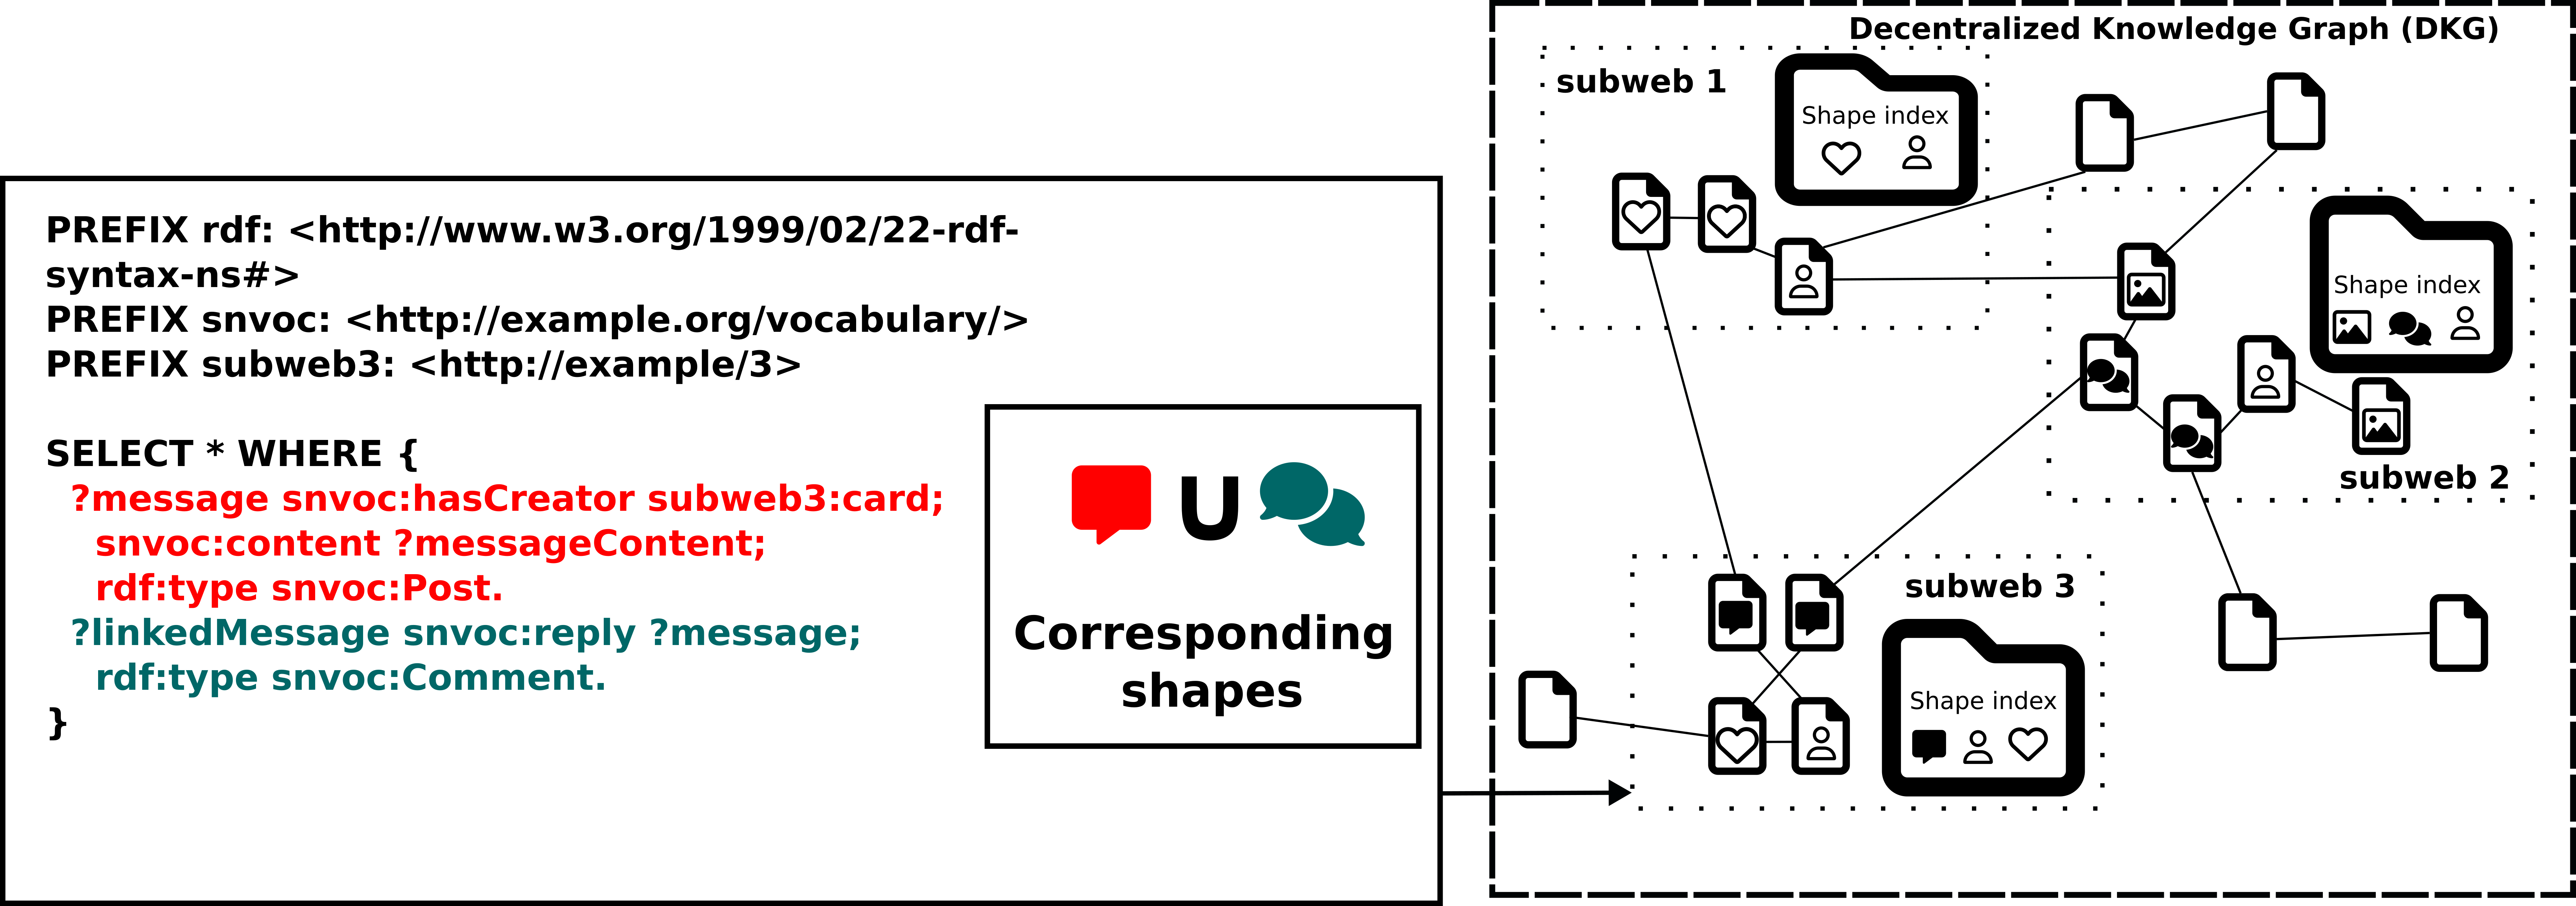
\includegraphics[width=0.80\textwidth]{figure/dkg.png}
   \caption{
      Given that the resources of a DKG are indexed with a shape index, a query engine can dereference a subset of the network.
      \jr{This should be a vector (e.g., SVG or PDF) image to avoid pixelation}
      %The nodes represent RDF resources, while the edges represent IRIs linking one resource to another (see Section \ref{sec:dkg}).
      %Each subweb has a shape index that maps shapes, represented by icons, to RDF resources by embedding the icon within the node.
      %The query engine starts its query at subweb 3, and the relevant query resources in a subweb are identified with a black node.
    }
    \label{fig:dkg}
\end{figure}

Our contributions include (i) a link pruning approach using shape indexes for LTQP; (ii) a novel query-shape subsumption algorithm for assessing data source relevance, and (iii) an experimental evaluation using a synthetic benchmark.
Concretely in this work, we pose the following research question: 
\textbf{Can LTQP use shape-based pruning in DKG networks to reduce query execution time while preserving result completeness?}
To address this question, we propose the following hypotheses:  
(\textbf{H1}) Shape indexes reduce the number of non-contributing data sources retrieved and the query execution time.  
(\textbf{H2}) The execution time of a query-shape subsumption algorithm is negligible in social media applications.  
(\textbf{H3}) Stricter shape constraints lead to a greater reduction in HTTP requests.  
(\textbf{H4}) Querying a network with more \emph{complete} shape indexes results in faster query execution.  
(\textbf{H5}) Performance gain can be acquired in networks with less shape index information.

The remiander of this paper is organized as follows: first, we discuss the \hyperref[sec:related_work]{related work} and present the \hyperref[sec:preliminaries]{preliminaries}.
We then describe our \hyperref[sec:approach]{approach}, followed by the \hyperref[sec:experiment]{experimental setup} and the \hyperref[sec:result]{discussion of results}.
Finally, we present our \hyperref[sec:conclusion]{conclusion}.
